\begin{frame}{Многоквантовый эксперимент ЯМР\footnote[frame]{
J. Baum, M. Munowitz, A. N. Garroway, and A. Pines, J. Chem. Phys. 83, 2015 (1985).}}

  \begin{figure}
    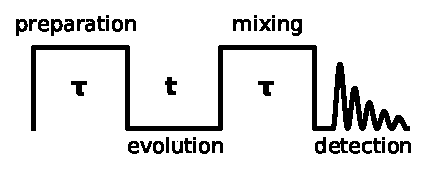
\includegraphics[width=0.5\textwidth]{mq-experiment-schema.pdf}
    %\caption{Схема МК эксперимента ЯМР}
  \end{figure}
  \vspace{-3mm}
  \begin{block}{}
    На подготовительном периоде МК эксперимента ЯМР система облучается последовательностью радиочастотных импульсов. В результате динамика спиновой системы определяется многоквантовым гамильтонианом.
    $$
    H_{MQ} = H^{(2)} + H^{(-2)},
    \quad H^{(\pm2)} = \frac 1 2 \sum_{i < j} D_{ij} I^\pm_i I^\pm_j
    \quad \rightarrow  \quad
    \rho_2 \sim I_{1z} I_{2}^{+} I_{3}^{+} I_{4z} I_{5}^{+} I_{6}^{-}
    $$
  \end{block}
\end{frame}
\note{
  В общем виде МК эксперимент ЯМР состоит из четырех периодов.
  На периоде подготовки спиновая система облучается периодической последовательностью резонансных радиочастотных импульсов. 
  В результате анизотропные диполь-дипольные взаимодействия становятся быстроосциллирующими,
  если обратный период облучающей последовательности значительно превосходит величину усредняемых взаимодействий. 
  Теория среднего гамильтониана позволяет найти усредненные взаимодействия, 
  гамильтониан которых несекулярный двухспиновый/двухквантовый гамильтониан $H_{MQ}$ ()

  Под действием этого гамильтониана матрица плотности может быть представлена в виде суммы вкладов когерентностей разных порядков. 

  Структура матрицы когерентности выглядит следующим образом, 
  разность между количеством повышающих и понижающих операторов определяют порядок когерентности. 

  Важной особенностью МК эксперимента ЯМР является то,
  что сигналы от когерентностей разных порядков можно разрешить. 
}

\begin{frame}{Многоквантовый экперимент ЯМР}
  \begin{columns}
    \column{0.4\textwidth}

    \begin{figure}
      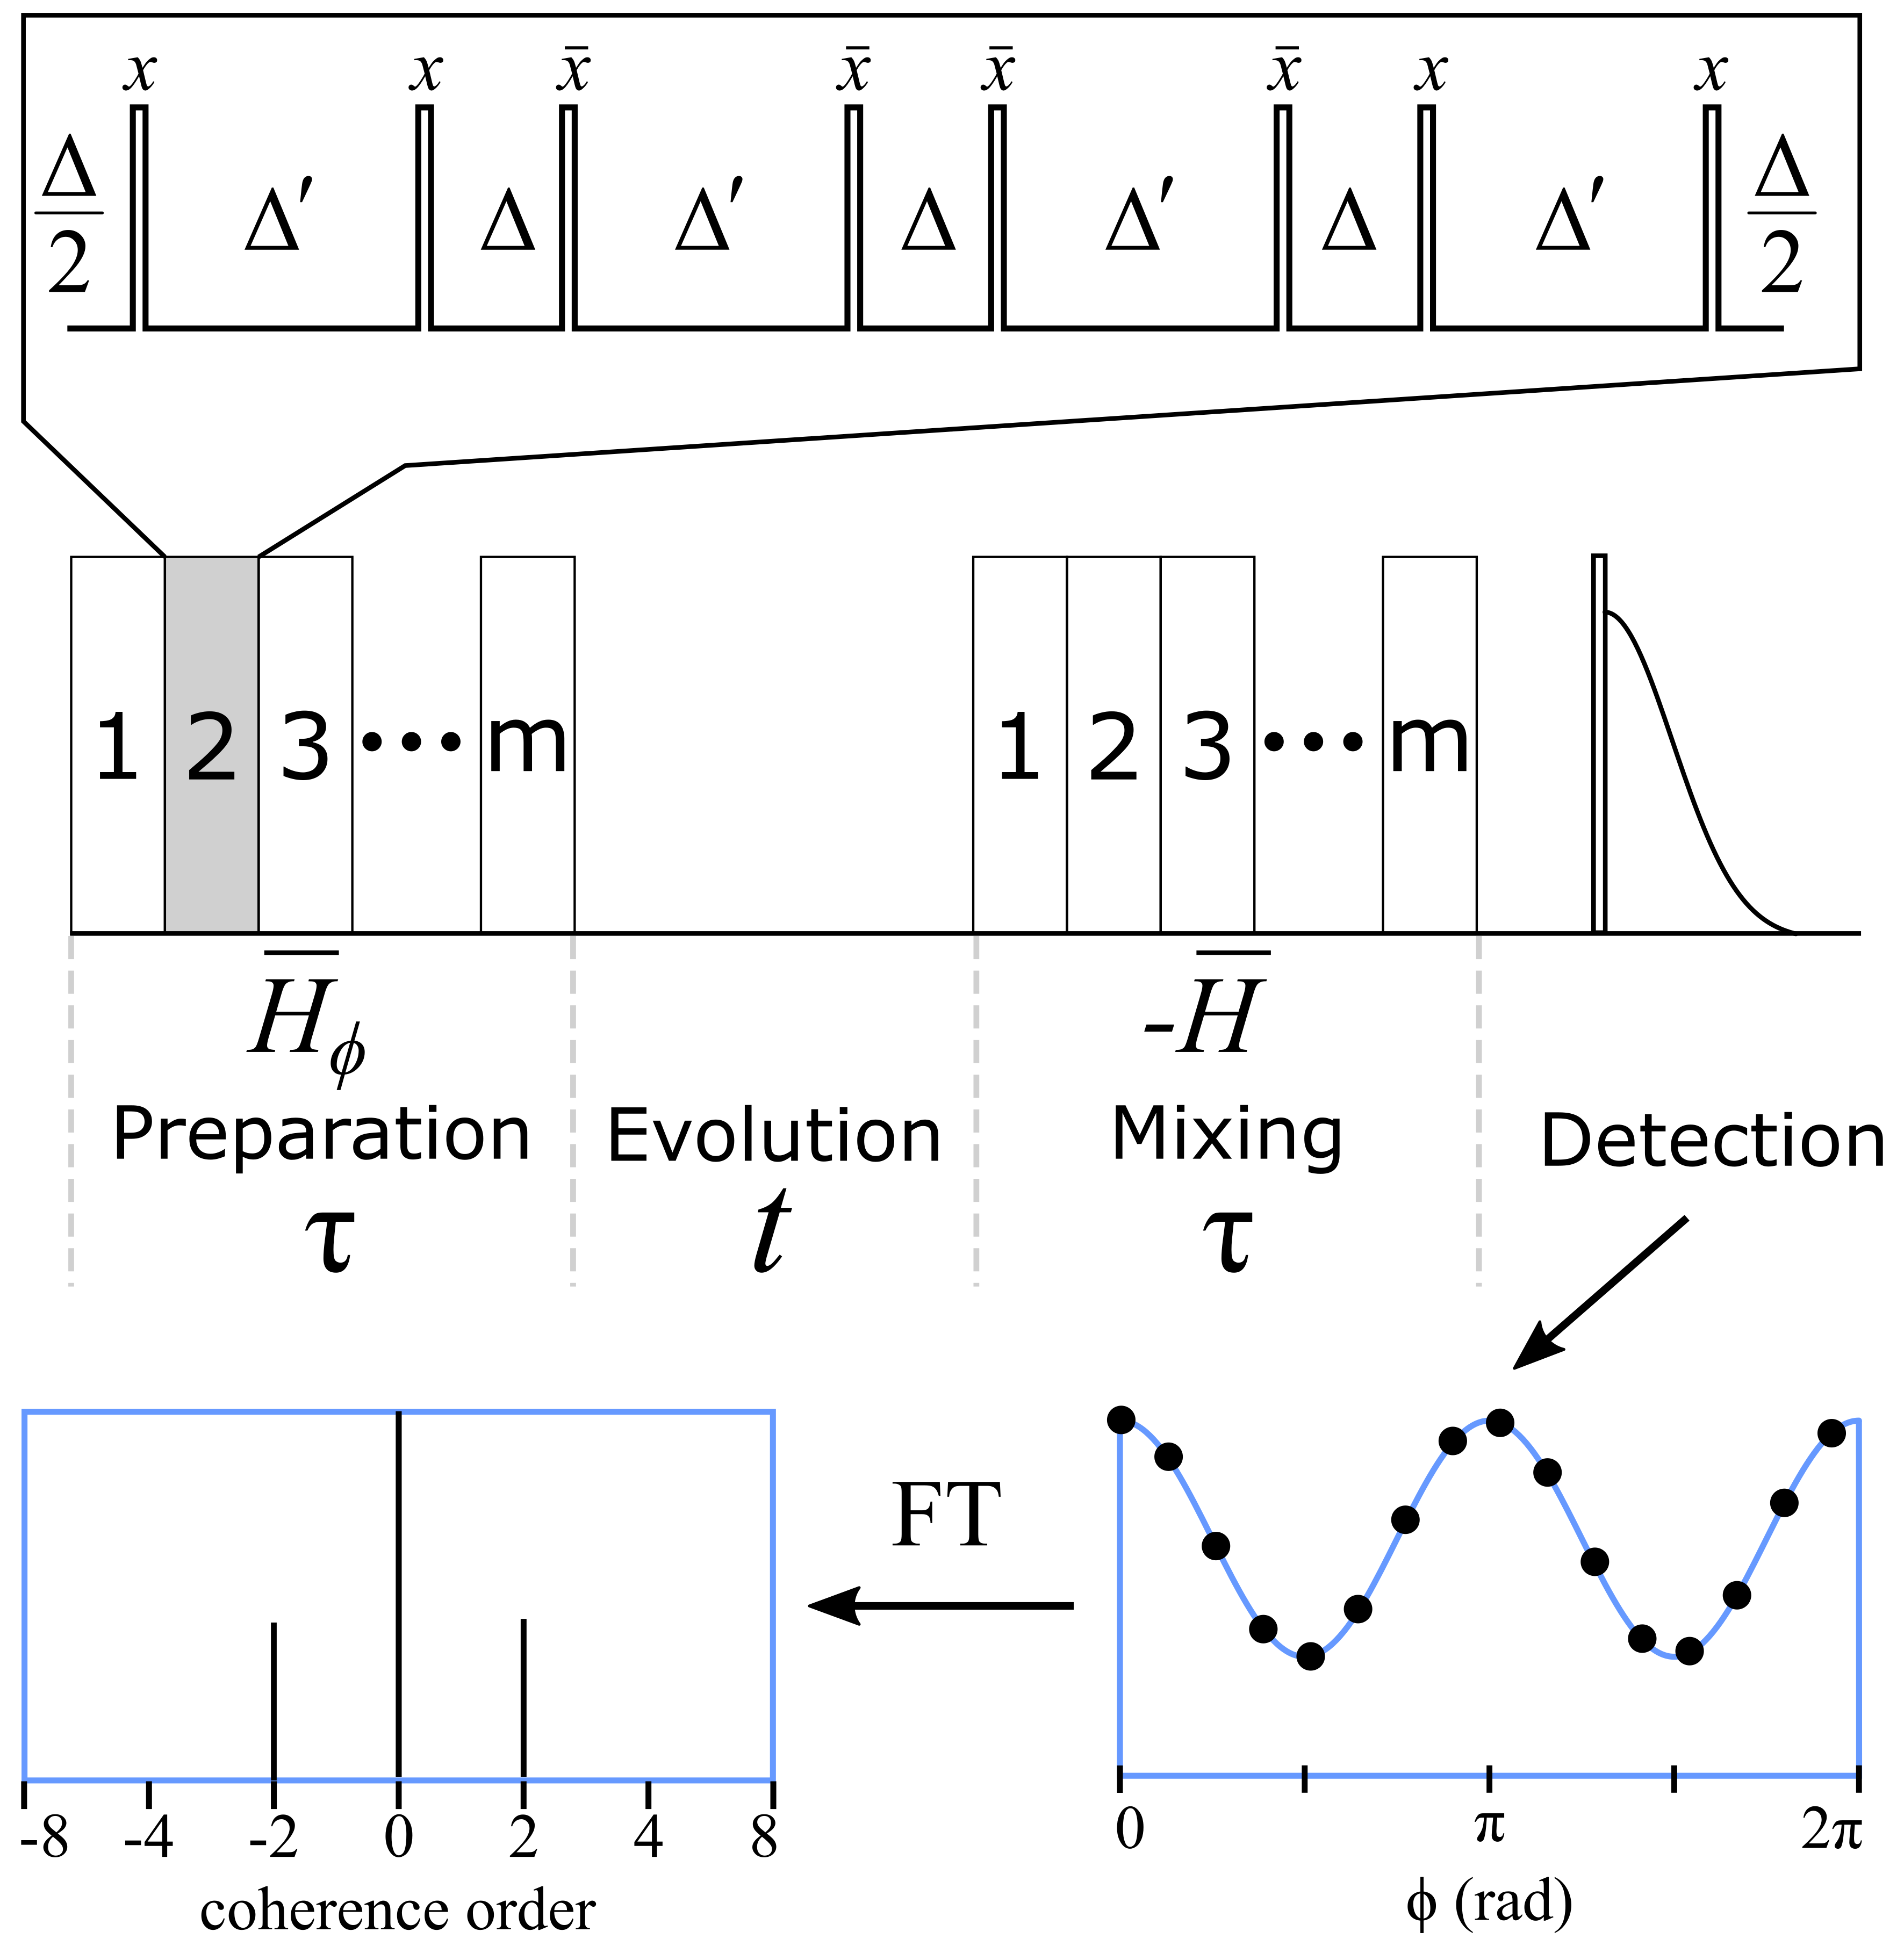
\includegraphics[width=0.9\textwidth]{mq-experiment-pulses-schema.png}
      \caption{Схематичное представление последовательности импульсов МК эксперимента.}
    \end{figure}


    \column{0.6\textwidth}
    МК когерентности создаются в течение периода подготовки продолжительностью $\tau$ при участии m-серии 8-импульсовых подпоследовательностей и затем преобразуются в наблюдаемую намагниченность после идентичного периода смешивания (за исключением 90-градусного фазового сдвига). Затем намагниченность детектируется при импульсе $\pi/2$. Фазовый сдвиг $\phi$ между периодами подготовки и смешивания инкриминируется для разделения многоквантовых когерентностей разных порядков. В результате преобразования Фурье по $\phi$ получается МК ЯМР спектр.
    % Интенсивности МК когерентностей ЯМР при различных длительностях периода свободной эволюции $t$ получаются в отдельных экспериментах.
  \end{columns}
\end{frame}
\note{
  Для разрешения сигналов когерентностей разных порядков. Периоды многократно повторяются с инкрементом фазы РЧ-импульсов, облучающих спиновую систему на подготовительном периоде при каждом повторении. 
  
  Поскольку многоквантовые когерентности ЯМР не могут наблюдаться непосредственно, они преобразуются в поперечную намагниченность (одно- квантовую когерентность) на периоде смешивания. На периоде смешивания спиновая система облучается такой же последовательностью РЧ-импульсов, как и на подготовительном периоде, но фаза им- пульсов сдвигается на $\pi$/2. (вместо x-импульсов подаются y-импульсы). 

  Детектирующий импульс подается для переноса намагниченности в плоскость, перпендикулярную внешнему магнитному полю. Затем записывается од- на точка, соответствующая максимальному значе- нию спада свободной индукции на временном интер- вале t2 для каждого инкремента фазы. 

  Преобразование Фурье относительно инкремента фазы позволя- ет получать многоквантовые спектры, состоящие из набора узких линий, отвечающих различным поряд- кам когерентностей. 
}
